\section{Forsøg 2 - IKEA-oplader} \label{sec:forsg2}

I dette forsøg undersøges sammenhængen mellem afstanden af oplader (senderen) og telefonen (modtageren) med henblik på tabet af energi når der sker en trådløs opladning med en QI certificeret oplader. Specifikt når afstanden $(L)$ mellem sender og modtager vokser. Altså effektiviteten $\eta$ undersøges ved forskellige afstande mellem sender og modtager.

\subsection{Forsøgsbeskrivelse} 
\subsubsection{Komponenter}

\begin{table}[htbp] %% Komponenter tabel %%
\begin{tabular}{l|l|c|l}
        & Strømforsyning               & Oplader             & Cover               \\ \hline
Model:  & KMW-190-330-GS               & MORIK, E1404        & VITAHULT, 22974     \\
Input:  & 220-240V$\sim$50/60Hz, 0.18A & 19V$\sim$1.74A, 33W & 5 W       \\	
Output: & 19V$\sim$1.74A, 10W          & 5W                  & 5V, 1A             
\end{tabular}
\caption{Alt er aflæst direkte fra komponenternes etiketter.}
\label{table:sender}
\end{table}

%%%%%%%%%%%%%

\begin{table}[htbp]
\begin{tabular}{l|lcl}
         & Iphone 4 &          &        \\ \hline
Batteri: & Li-Po     & 1420 mAh & 5,3 Wh
\end{tabular}
\caption{Aflæst fra \cite{batteri}}
\label{table:batteri}
\end{table}

Strømkilden til strømforsyningen er et standart ikke jordet, tobenet, europæisk væg stikkontakt, 230 volt 50 Hz.

Som modtager er der benyttet en \textbf{Iphone 4}, \textit{Model A1332 EMC 380A med FCC ID: BCG-E2380A, IC: 579C-E2380A.}\footnote{Aflæst fra bagsiden af enheden.}
Denne enhed er udstyret med cover, model og egenskaber kan ses i tabel \ref{table:sender}. Her er det dog vigtigt at notere sig at telefonen er brugt, og er en ældre model (købt november 2011). Altså er batteriet ikke i fabriksny tilstand. Det er usikkert om dette har haft en relevant effekt på det udførte forsøg. Da dette kan have en effekt på hvordan batteriet lader. I forsøget er der antaget at opladningen sker lineært, mere om dette i følgende sektioner.

Ydermere er der benyttet papir til at lægge imellem mobilen med coveret og opladeren for at øge afstanden mellem dem, så det magnetiske felt forstyrres mindst muligt, og afstanden er holdt fast. 

\begin{figure}
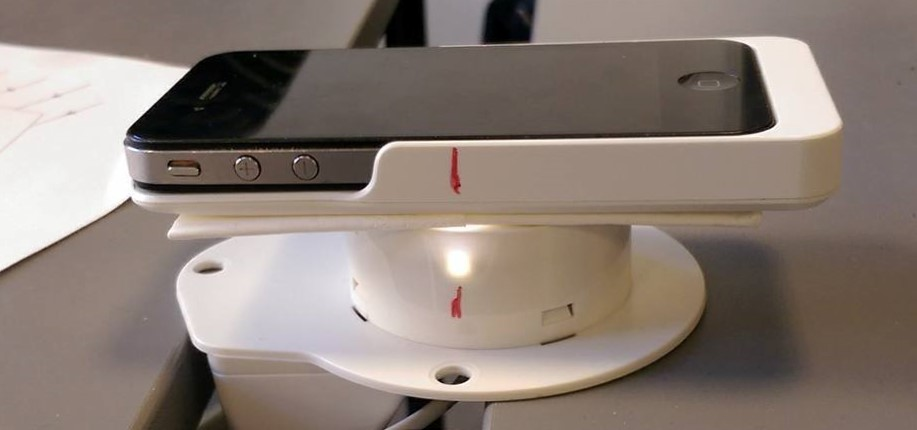
\includegraphics[width=1\textwidth]{Vildledning/Schematics/forsg2_opstilling1}
\caption{Opstilling med Iphone 4 og IKEA oplader L = 0,25 cm}
\label{figure:opstilling}
\end{figure}

\subsubsection{Fremgangsmåde}

Udførelsen af forsøget er meget simpel, og består af to dele der gentages tre gange. Første del er at bestemme hvor højt modtager telefonen skal være løftet fra opladeren. Altså længden L bestemmes i cm, hvor positiv retning er væk fra opladeren. Anden del er at aflæse telefonens batteriprocent hvert tiende minut. Dette gentages med tre forskellige værdier for L, altså tre forskellige afstande.

Alle tre gange sikres der at koblingen ikke er ustabil. Hjælp til at opnå dette er en diode, i opladeren, der lyser konstant hvis koblingen er stabil. For at opnå denne stabile kobling placeres telefonen midt ovenpå opladeren, så spolerne i henholdsvis sender og modtager ligger direkte ovenpå hinanden. Hertil er der tegnet en rød streg på både oplader og cover, det det er muligt at afgøre at coveret ligger samme sted under hvert forsøg.

Første L værdi er valgt til 0 cm da dette teoretisk set burde være den optimale kobling mellem sender og modtager i et system designet til trådløs energioverførsel. Det ses også i den første graf der hvor $L = 0$ at denne opnår den højeste ladningsprocent. Det skal dog noteres at spolerne i sender og modtager ikke lægger præcist direkte ovenpå hinanden da der er et lag plastik og et gummikryds imellem. Disse antages ikke at have nogen effekt på opladningen. Længden L starter fra den hvide plastikskive med gummikrydset på opladeren, altså direkte ovenpå. Den præcise afstand mellem plastic og spole i senderen er ukendt. Det samme gælder i coverets ydre plastiklag, hvor dennes tykkelse og afstand mellem den og modtager spolen også er ukendt.

Tiden er målt hvert tiende minut (bilag \ref{bilag:forsg2}) og målt med en afvigelse på $\pm 5$ sekunder, hvilket burde være hurtigt nok til ikke at se en ændring i ladningsprocenten.

Til slut undersøges værdien af L hvor der ikke er muligt at danne en kobling, altså der hvor dioden stopper med at lyse og der ikke sker en opladning af batteriet.

\subsubsection{Resultater}
Det ses at op til omkring L = 1 cm, at det ikke er muligt at danne en forbindelse mellem opladeren og coveret med telefonen i.

Rå, ikke redigeret, data kan ses i bilag \ref{bilag:forsg2}. Disse data er benyttet til at opstille de følgende tre diagrammer:

\begin{figure}[H]
\centering
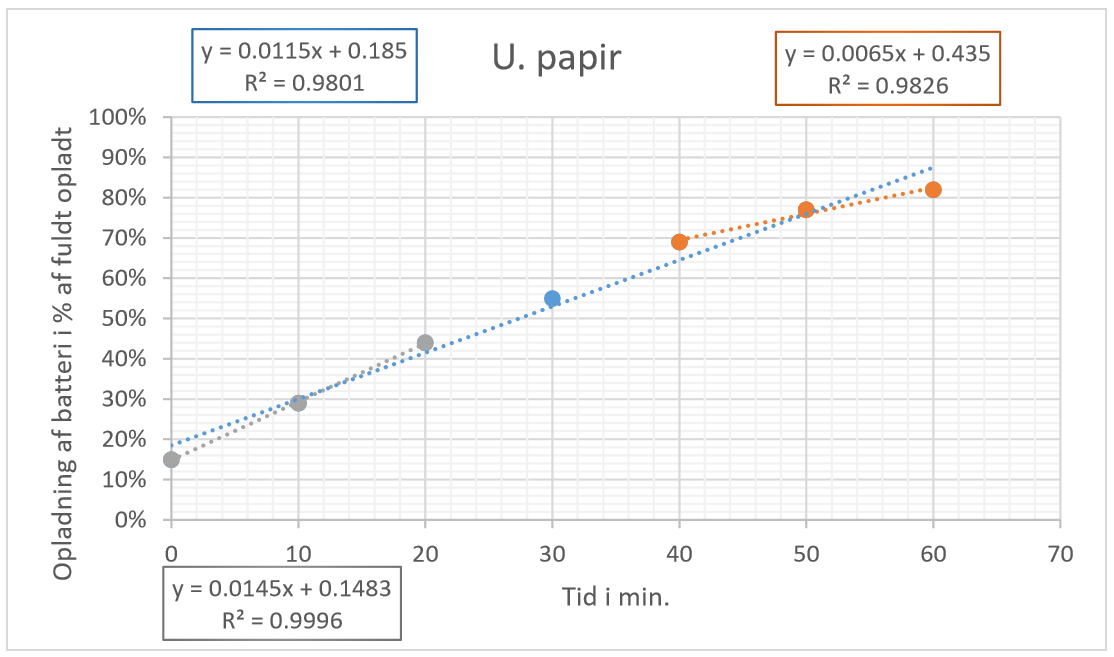
\includegraphics[width=1\textwidth]{Setup/forsg2_graf1}
\caption{}
\label{figure:graf1}
\end{figure}

\begin{figure}[H]
\centering
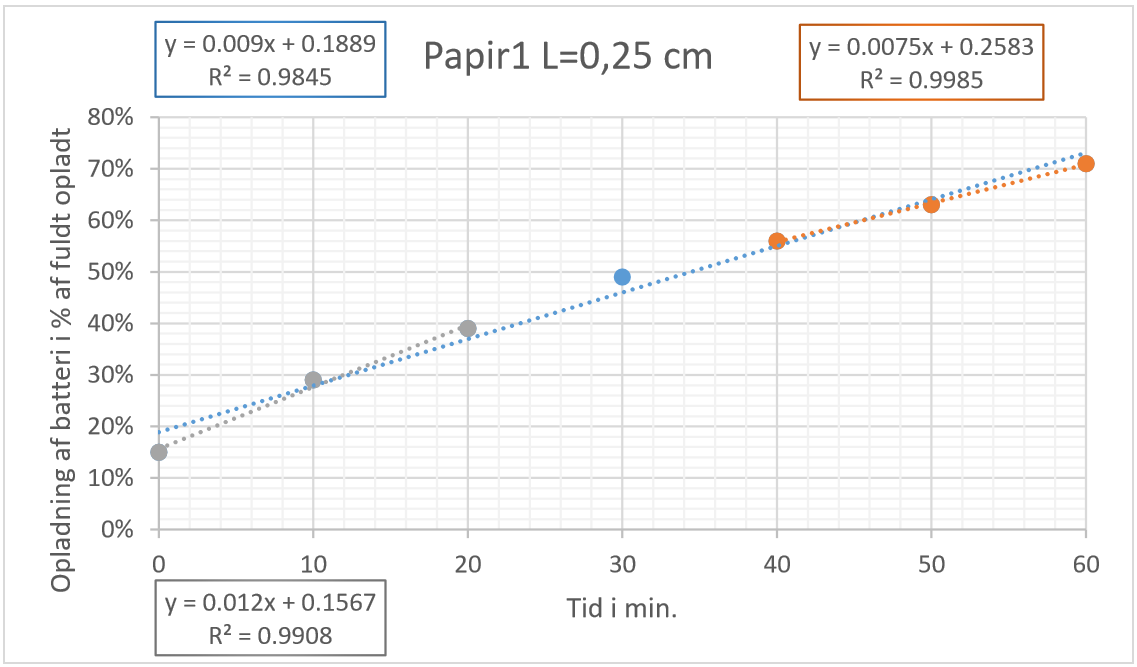
\includegraphics[width=1\textwidth]{Setup/forsg2_graf22}
\caption{}
\label{figure:graf2}
\end{figure}

\begin{figure}[H]
\centering
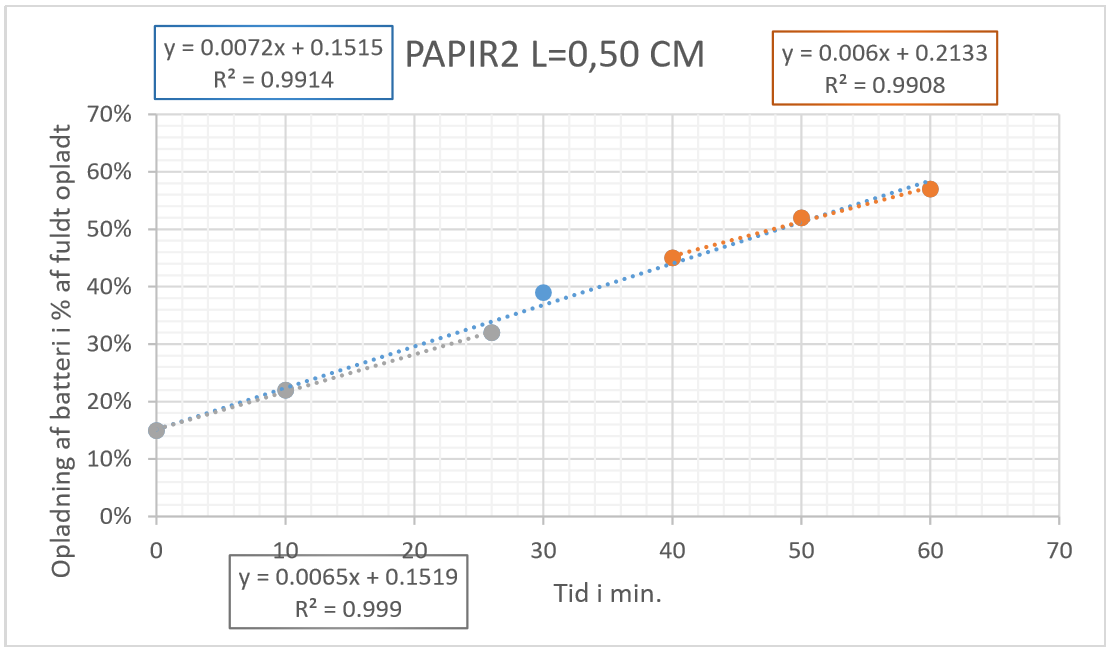
\includegraphics[width=1\textwidth]{Setup/forsg2_graf3}
\caption{}
\label{figure:graf3}
\end{figure}

I første forsøg hvor $L = 0$ ses det at opladning af batteriet nåede op på 82 procent ladning af maksimal ladning på batteriet (100 procent), indenfor den målte tidsperiode på 60 minutter. I de to næste forsøg ender opladningsprocenten efter 60 minutter på henholdsvis 81 procent og 57 procent ved $L = 0.25$ og $L = 0.5$ aflæst fra datasættet i bilag \ref{bilag:forsg2} og ses tydeligt på figur \ref{figure:graf1}, figur \ref{figure:graf2} og figur \ref{figure:graf3}.

Der er lavet tre lineære regressioner per diagram, en af de tre førstedatapunkter en for de tre sidste og den over dem alle samlet. Her ses det at opladningen ikke sker helt lineært, altså at opladningen sker ved samme hastighed gennem hele forløbet. Ved sammenligning af hældningskoefficienten af de tre første punkter og tre sidste punkter ses det at opladningen er mere effektiv i starten af opladningen end den er til slut f.eks. i figur \ref{figure:graf1} hvor $0,012\, \frac{E_\%}{t} > 0,009\, \frac{E_\%}{t}$.

Den ikke lineære opladning kan skyldes af et væld af ting, hvor det er antaget at det ikke er skyldt af den trådløse opladning, men snarere faktorer som: et ældre batteri, smartchargin teknologi\footnote{Det er ikke undersøgt om den målte telefon har disse teknologier eller hvordan de fungerer, på højere end basis niveau.} eller andet software der har en effekt på batteriet el. andet. 

\subsection{Databehandling}
I denne sektion undersøges det, ud fra det begrænsede datasæt, hvor stor effektivitet der mistes ved at forlænge afstanden mellem oplader og telefon med cover. Dette undersøges ved at beregne forskellige nyttevirkninger for den varierende værdi af L. 

Det antages at når batteriets batteri procent kan aflæses til 100 \% på telefonens display at batteriet indeholder $O_{maks}=1432\, mAh \approx 5,3 Wh$. Dette benyttes så til at udregne nyttevirkningen $\eta$ med watt time værdier.

Det aflæses i skemaet \ref{table:sender} at opladeren har en effekt på 5 W og coveret har en en effekt på $(5 V \cdot 1 A = 5 W)$. Hvis det antages at der bliver ladt op telefonens batteri med den fulde mulige effekt gennem hele forsøget (lineær opladning) kan der bestemmes hvilken procent batteriet skulle kunne aflæses til efter 60 minutter:

\begin{equation}
O_{maks60}= \frac{5 W\cdot 1h}{5,3Wh} \cdot 100 \approx 94 \%
\label{eq:omaks}
\end{equation}

Dette er så den teoretiske maksimale opladningsprocent batteriet kan ende på. Denne viser også hvor meget der kan lades på batteriet på 60 minutter:
\begin{equation}
\Delta O_{maks} = 5 W \cdot 1 h = 5Wh
\end{equation}

Altså er den maksimale mængde watt timer den givne oplader kan påføre batteriet 5. I alle forsøgene starter mobilen på 15 \% opladning af de 5,3 Wh så:
\begin{align*}
O_{start} = 5,3 \cdot 0,15 = 0,8 Wh
\end{align*}
 

\textbf{1. kør (L=0)}

I det første forsøg ender telefonen på 82 \% efter 60 minutter så:
\begin{align*}
& \Delta O_{1\%} = 82\%-15\% =  67\%  \\
& \Delta O_1 = 5,3 Wh \cdot 0,67 = 3,6 Wh
\end{align*}


Nyttevirkningen (i \%) kan nu beregnes vha. $\Delta O_1$ og $\Delta O_{maks}$:  
\begin{equation}
\eta_1 = \frac{\Delta O_1}{\Delta O_{maks}} \cdot 100 = \frac{3,6 Wh}{5 Wh} \cdot 100 \approx 86 \%
\label{eq:nyt1}
\end{equation}

Dette gøres ved de to næste forsøg, stadig efter 60 minutters opladning.

\textbf{2. kør (L=0,25):}
\begin{align*}
& \Delta O_{2\%} = 71\%-15\% =  56\%  \\
& \Delta O_2 = 5,3 Wh \cdot 0,56 = 3 Wh
\end{align*}
Nyttevirkningen beregnes:
\begin{equation}
\eta_2 = \frac{\Delta O_2}{\Delta O_{maks}} \cdot 100 = \frac{3 Wh}{5 Wh} \cdot 100 = 60 \%
\label{eq:nyt2}
\end{equation}

\textbf{3. kør (L=0,5):}
\begin{align*}
& \Delta O_{3\%} = 57\%-15\% =  42\%  \\
& \Delta O_3 = 5,3 Wh \cdot 0,42 = 2,2 Wh
\end{align*}
Nyttevirkningen beregnes:
\begin{equation}
\eta_3 = \frac{\Delta O_3}{\Delta O_{maks}} \cdot 100 = \frac{2,2 Wh}{5 Wh} \cdot 100 \approx 44 \%
\label{eq:nyt3}
\end{equation}

De tre værdier for $\eta$ stilles op i et $(L,\eta)$ koordinatsystem ser det således ud som i figur \ref{figure:graf4}

\begin{figure}[H]
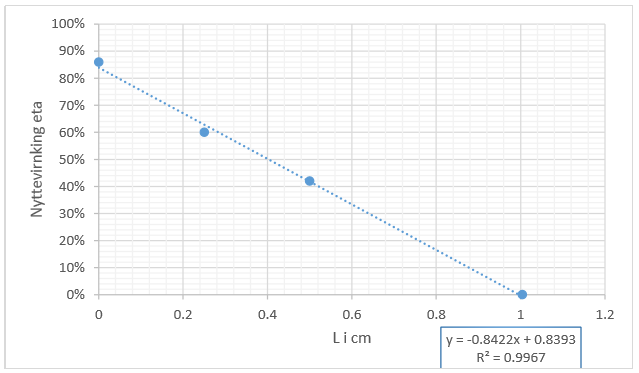
\includegraphics[width=1\textwidth]{Setup/forsg2_graf4}
\caption{}
\label{figure:graf4}
\end{figure}
I samme omgang laves der en lineær regression men kun af de tre målte punkter, dette aflæses til:
\begin{equation}
y=-0,8422x+0,8393 \Rightarrow \eta = -0,8422L+0,8393
\label{eq:regression}
\end{equation}
Det sidste punkt der er skæringen med x-aksen bestemmes ud fra regressionen \ref{eq:regression}:
\begin{align*}
& solve(\eta =-0.8422L+0.8393,L) \\
& \Leftrightarrow L = 1,003964 \approx 1 cm
\end{align*} 
Dette er så den maksimale værdi for L, altså den maksimale afstand mellem opladerens overflade og telefonen med cover. Dette virker som en brugbar projektion da det er tæt på den maksimale L værdi som der blev målt til under forsøget, der var lige under 1 cm. Dette vil så sige at den bestemte lineære ligning til en vis grænse kan benyttes til at vise en sammenhæng mellem afstanden og nyttevirkningen, og i sidste ende hvor meget power man kan få ud af opladeren. I hvert fald for den givne IKEA oplader.

Altså i de tre forsøg formåede den trådløse oplader fra IKEA at overføre 3,6 Wh, 3,0 Wh og 2,2 Wh som henholdsvis er en nyttevirkning på 86 \%, 60 \% og 44 \% for de tre forsøg. Altså er det tydeligt at når afstanden L mellem sender og modtager vokser mindskes energioverførslen betydeligt. Ud fra de tre forsøg og den dannede prognose ses det at den benyttede IKEA (QI) opladers nyttevirkning ændrer sig ud fra ligning \ref{eq:regression}.